\documentclass[aspectratio=169, handout]{beamer}

%########################################################
%####################### SET THEME
%########################################################
\usetheme{Goettingen}
\setbeamertemplate{footline}[frame number]

%########################################################
%##################### ADD PACKAGES
%########################################################
\usepackage{tabularx}
\usepackage{amsmath}
\usepackage{amsfonts}
\usepackage{amssymb}
\usepackage{etoolbox,refcount}
\usepackage{multicol}

%########################################################
%################## ARGMAX DECLARATION
%########################################################
\DeclareMathOperator*{\argmax}{arg\,max}

%########################################################
%############ AUTOMULTICOLITEMIZE ENVIRONMENT
%########################################################
\newcounter{countitems}
\newcounter{nextitemizecount}
\newcommand{\setupcountitems}{%
  \stepcounter{nextitemizecount}%
  \setcounter{countitems}{0}%
  \preto\item{\stepcounter{countitems}}%
}
\makeatletter
\newcommand{\computecountitems}{%
  \edef\@currentlabel{\number\c@countitems}%
  \label{countitems@\number\numexpr\value{nextitemizecount}-1\relax}%
}
\newcommand{\nextitemizecount}{%
  \getrefnumber{countitems@\number\c@nextitemizecount}%
}
\newcommand{\previtemizecount}{%
  \getrefnumber{countitems@\number\numexpr\value{nextitemizecount}-1\relax}%
}
\makeatother    
\newenvironment{AutoMultiColItemize}{%
\ifnumcomp{\nextitemizecount}{>}{3}{\begin{multicols}{2}}{}%
\setupcountitems\begin{itemize}}%
{\end{itemize}%
\unskip\computecountitems\ifnumcomp{\previtemizecount}{>}{3}{\end{multicols}}{}}


%########################################################
%###################### TITLE PAGE
%########################################################
\title{An Experience with Text Classification in \textit{Datadays 2019}}
\author{Majid Hajiheidari \and Amirmohammad Asadi}
\date{April, 2019}

%########################################################
%####################### DOCUMENT
%########################################################
\begin{document}
	\frame{\titlepage}
	\section{Introduction: Divar Dataset}
	\frame{
		\frametitle{Divar Posts Dataset}
		\begin{columns}
			\begin{column}{.5\textwidth}
				\begin{itemize}
					\item<2-> Released for DataDays 2019
					\item<3-> One million posts
				\end{itemize}
			\end{column}
			\begin{column}{.5\textwidth}
				%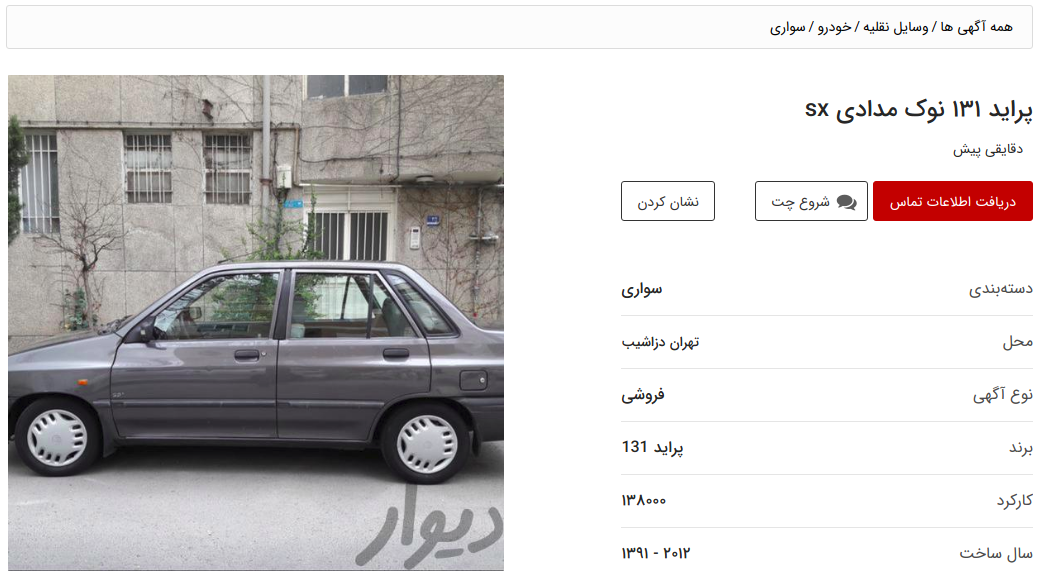
\includegraphics[height=\linewidth]{images/post1.png}
				
\includegraphics[width=\linewidth]{images/post2.png}
				
\includegraphics[width=\linewidth]{images/post3.png}
			\end{column}
		\end{columns}		
	}
	\frame{
		\frametitle{Columns}
		\begin{AutoMultiColItemize}
			\item id
			\item archive\_by\_user
			\item published\_at
			\item  \textbf <2> {cat1}
			\item  \textbf <2> {cat2}
			\item  \textbf <2> {cat3}
			\item city
			\item  \textbf <2> {title}
			\item  \textbf <2> {desc}
			\item price
			\item image\_count
			\item platform
			\item mileage
			\item brand
			\item year
			\item type
		\end{AutoMultiColItemize}
	}
%	\frame{
%		\frametitle{Title, Description, and Category}
%		\begin{tabular}{l|l|l|l|l}
%			\textbf{Title} & \textbf{Description} & \textbf{Cat1} & \textbf{Cat2} & \textbf{Cat3}\\
%			\hline
%			1&2&3&4&5
%		\end{tabular}
%		\\Some text
%	}
	\section{The Problem: Categorization}
		\frame{
			\frametitle{The Problem: Categorization}
			\begin{itemize}
				\item <2-> We need to categorize posts based on other posts features;
				\item <3-> We only use text features(title \& description)!
			\end{itemize}
		}
		%\subsection{Features}
			\frame{
				\frametitle{Features}
				This slide is temp.
			}
		%\subsection{No. of Classes}
			\frame{
				\frametitle{No. of Classes}
				This slide is temp.
			}
	\section{Feature Extraction}
	\frame{
		\frametitle{Feature Extraction}
		Feature extraction is a dimensionality reduction process, where an initial set of raw variables is reduced to more manageable groups (features) for processing, while still accurately and completely describing the original data set.
	}
		\subsection{Count Vectorizer}
		\frame{
				\frametitle{Vectorizing the Text: Count Vectorizer}
				An example: We want to vectorize these 4 setences\footnote{Example from \href{https://github.com/rahulvasaikar/Bag-of-words}{Rahul Vasaikar}}:\\
				\begin{enumerate}
					\item Hello, how are you!
					\item Win money, win from home.
					\item Call me now
					\item Hello, Call you tomorrow?
				\end{enumerate}
			}
			\frame{
				\frametitle{Vectorizing the Text: Count Vectorizer}
				\begin{enumerate}
					\item We first build a vocabulary:\\
					\begin{math}
					vocabulary = \left\{are, call, from, hello, home, how, me, money, now, tomorrow, win, you\right\}
					\end{math}
					\item Then, we vectorize each sentence based on the occurness of each word:
					\scriptsize\begin{tabular}{l|llllllllllll}
						& are & call & from & hello & home & how & me & money & now & tom... & win & you \\\hline
						1       & 1   & 0    & 0    & 1     & 0    & 1   & 0  & 0     & 0   & 0        & 0   & 1   \\
						2 & 0   & 0    & 1    & 0     & 1    & 0   & 0  & 1     & 0   & 0        & 2   & 0   \\
						3               & 0   & 1    & 0    & 0     & 0    & 0   & 1  & 0     & 1   & 0        & 0   & 0   \\
						4 & 0   & 1    & 0    & 1     & 0    & 0   & 0  & 0     & 0   & 1        & 0   & 1  
					\end{tabular}
				\end{enumerate}
			}
			\frame{
				\frametitle{Vectorizing the Text: Count Vectorizer}
				N pair of samples
			}
		\subsection{Tf-idf Vectorizer}
		\frame{
			\frametitle{Tf-idf Vectoizer}
			\begin{itemize}
				\item Tf-idf stands for term frequency-inverse document frequency
				\item a statistical measure used to evaluate how important a word is to a document in a collection or corpus
				\item the tf-idf weight is composed by two terms:
					\scriptsize\begin{description}
						\item [TF] \textbf{Term Frequency}, which measures how frequently a term occurs in a document.
						\begin{equation*}
						TF(t) = \frac{Number\ of\ times\ term\ t\ appears\ in\ a\ document}{Total\ number\ of\ terms\ in\ the\ document}
						\end{equation*}
						\item [IDF] \textbf{Inverse Document Frequency}, which measures how important a term is
						\begin{equation*}
						IDF(t) = \ln{\frac{Total\ number\ of\ documents}{Number\ of\ documents\ with\ term\ t\ in\ it}}
						\end{equation*}
					\end{description}
			\end{itemize}
		}
		\frame{
			\frametitle{Tf-idf Vectorizer: An Example}
			Consider a document containing 100 words wherein the word \textit{cat} appears 3 times. The term frequency (i.e., tf) for cat is then $tf(cat) = \frac{3}{100} = 0.03$. Now, assume we have 10 million documents and the word cat appears in one thousand of these. Then, the inverse document frequency (i.e., idf) is calculated as $idf(cat) = \ln{\frac{10,000,000}{1,000} = 4}$. Thus, the Tf-idf weight is the product of these quantities: $tf\--idf(cat) = 0.03 * 4 = 0.12$.
		}
		\subsection{Embedding}
		\frame{
			\frametitle{Temp Frame}
			This slide is temp.
		}
		
	\section{Classification Algorithms}
	\frame{
		\frametitle{Classification Algorithms}
		We used different classifiers and applied different models on the data. The classifiers we tested are:
			\begin{itemize}
				\item Naive Bayes
				\item Linear Support Vector Machine(SVM)
				\item Passive Aggressive
				\item Convolutional Neural Network(CNN)
			\end{itemize}
	}
		\subsection{Naive Bayes}
		\frame{
			\frametitle{Naive Bayes Classifier}
			\begin{columns}
				\begin{column}{.5\textwidth}
					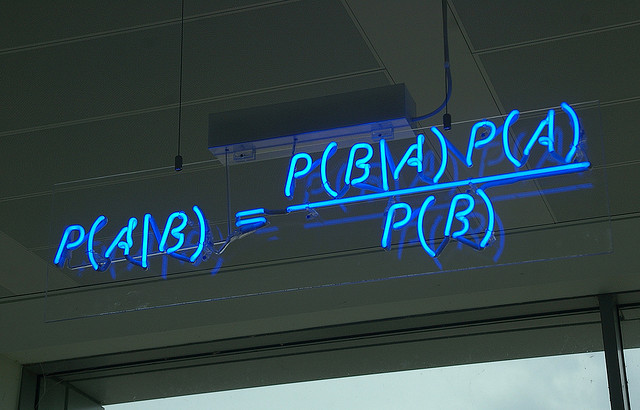
\includegraphics[width=\linewidth]{images/bayes_formula.jpg}
					\begin{center}
						Photo by \href{https://www.flickr.com/photos/mattbuck007/3676624894}{Matt Buck}
					\end{center}
				\end{column}
				\begin{column}{.5\textwidth}
					\begin{center}
						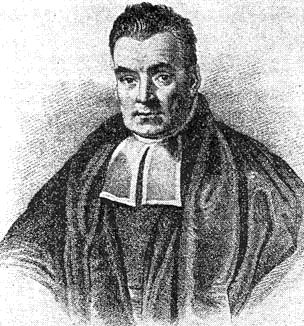
\includegraphics[width=.8\linewidth]{images/Thomas_Bayes.png}
					\end{center}
				\end{column}
			\end{columns}
		}
		%\subsection{Count Vectorizer}
			
		%\subsection{Bayes Classifier}
			\frame{
				\frametitle{Bayes Classifier: Naive One!}
				It is possible to show that accuracy is minimized, on average, by a
				very simple classifier that assigns each observation to the most likely class,
				given its predictor values. In other words, we should simply assign a test
				observation with predictor vector $x_0$ to the class j for which\\
				\begin{center}
					\begin{math}
						P\left(Y=j\ \middle|\ \mathbf{X}=\mathbf{x}\right)
					\end{math}
				\end{center}
				is largest.
			}
			\frame{
				\frametitle{Bayes Classifier: Naive One!}
				We make two assumptions:
				\begin{enumerate}
					\item $X_1, X_2, \ldots, and\ X_m$ are independent from each other;
					\item $X_1, X_2, \ldots, X_m\mid Y \thicksim MN(\cdot, p_1, p_2, \ldots, p_m)$
				\end{enumerate}
				{\scriptsize\begin{align*}
					P(Y=j\mid\mathbf{X}=(x_1, x_2, \ldots, x_m))
					 &= \frac{P(\mathbf{X}=(x_1, x_2, \ldots, x_m)\mid Y=j)\cdot P(Y=j)}{P(\mathbf{X}=\mathbf{x})}\\
					 &= \frac{P(X_1=x_1\mid Y=j)\cdot\ldots\cdot P(X_m=x_m\mid Y=j)\cdot P(Y=j)}{P(\mathbf{X}=\mathbf{x})}.
				\end{align*}}
				\scriptsize\begin{align*}
					\hat{y} = \argmax_{j\in classes} \frac{P(X_1=x_1\mid Y=j)\cdot\ldots\cdot P(X_m=x_m\mid Y=j)\cdot P(Y=j)}{P(\mathbf{X}=\mathbf{x})}\\
					=\argmax_{j\in classes} P(X_1=x_1\mid Y=j)\cdot\ldots\cdot P(X_m=x_m\mid Y=j)\cdot P(Y=j).
				\end{align*}
			}
			\frame{
				\frametitle{Bayes Classifier: Naive One!}
				Let's dive into code!
			}
		%\subsection{Hyperparameters}
			\frame{
				\frametitle{Hyperparameters}
				Two important hyperparameters:
				\begin{enumerate}
					\item Size of the vocabulary;
					\item Laplace/ Lidstone smoothing parameter($\alpha$).
				\end{enumerate}
			}
			\frame{
				\frametitle{Size of Vocabulary}
				\begin{center}
					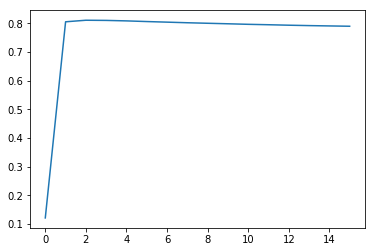
\includegraphics[width=.6\linewidth]{images/plot1.png}\\
					It is convex!
					(to be completed)
				\end{center}
			}
			\frame{
				\frametitle{Laplace/ Lidstone Smoothing Parameter($\alpha$)}
				\begin{center}
					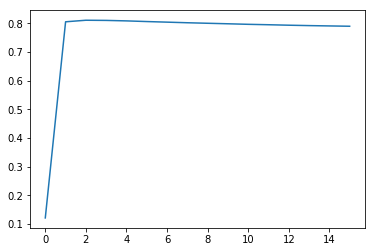
\includegraphics[width=.6\linewidth]{images/plot1.png}\\
					It is convex!
					(to be completed)
				\end{center}
			}
			\frame{
				\frametitle{Grid Search}
			}
		\subsection{CNN}
	%\section{First approach: Naive Bayes}
		
	%\section{Second approach: CNN}
		%\subsection{Sequence of vectors}
			\frame{
				\frametitle{Temp Frame}
				This slide is temp.
			}
		%\subsection{How We Embed}
			\frame{
				\frametitle{Temp Frame}
				This slide is temp.
			}
		%\subsection{Patterns with CNN}
			\frame{
				\frametitle{Temp Frame}
				This slide is temp.
			}
		%\subsection{Dense Classifier}
			\frame{
				\frametitle{Temp Frame}
				This slide is temp.
			}
		\subsection{Linear SVM}
		\frame{
			\frametitle{Linear SVM}
			\begin{itemize}
				\item A non-probablistic classifier
				\item A discriminative classifier formally defined by a separating hyperplane
				\item The algorithm outputs an optimal hyperplane which categorizes new examples
				\item A good separation is achieved by the hyperplane that has the largest distance to the nearest training-data point of any class
			\end{itemize}
		}
		\frame{
			\frametitle{Linear SVM: Behind the Scene}
			Given training vectors $x_i \in \mathbb{R}^p$, i=1,...,n, in two classes, and a vector $y \in \{1, -1\}^n$, SVM classifier solves the following primal problem:
			\scriptsize \begin{align*}
			\begin{aligned}
			\min_ {w, b, \zeta} \frac{1}{2} w^T w + C \sum_{i=1}^{n} \zeta_i\\\begin{split}\textrm {subject to } & y_i (w^T \phi (x_i) + b) \geq 1 - \zeta_i,\\& \zeta_i \geq 0, i=1, ..., n\end{split}
			\end{aligned}
			\end{align*}
			\normalsize Its dual is:
			\scriptsize \begin{align*}
			\begin{aligned}
			\min_{\alpha} \frac{1}{2} \alpha^T Q \alpha - e^T \alpha\\
			\begin{split}\textrm {subject to } & y^T \alpha = 0\\& 0 \leq \alpha_i \leq C, i=1, ..., n
			\end{split}
			\end{aligned}
			\end{align*}
		}
		\frame{
			\frametitle{Linear SVM: Behind the Scene(cont'd)}
			where $e$ is the vector of all ones, $C > 0$ is the upper bound, $Q$ is an $n$ by $n$ positive semidefinite matrix, $Q_{ij} \equiv y_i y_j K(x_i, x_j)$, where $K(x_i, x_j) = \phi (x_i)^T \phi (x_j)$ is the kernel. Here, training vectors are implicitly mapped into a higher (maybe infinite) dimensional space by the function $\phi$. The decision function is:
			\begin{equation*}
			\operatorname{sgn}(\sum_{i=1}^n y_i \alpha_i K(x_i, x) + \rho)
			\end{equation*}
		}
		\subsection{Passive Aggressive}
		\frame{
			\frametitle{Temp Frame}
			This slide is temp.
		}
			
	\section{A Comparison among Models}
	
	\section{The End}
	\frame{
		\frametitle{Thanks for your attention!}
		Codes in slides (in my GitHub):(github link)\\
		Divar posts dataset:(divar link)\\
		Any questions?\\
		
	}
\end{document}